\documentclass[12pt]{report}
\usepackage[a4paper,left=35mm,right=20mm,top=25mm,bottom=25mm]{geometry} 
\usepackage[T1]{fontenc}
\pagestyle{plain}
\parindent 1cm
\def\baselinestretch{1.25}
\usepackage[table,xcdraw]{xcolor}
\usepackage{indentfirst}
\usepackage[font=small]{caption}
\usepackage{pdfpages}
\usepackage{float}
\usepackage[polish]{babel}
\usepackage{polski}
\usepackage[utf8]{inputenc}
\usepackage{tikz}
\usepackage{algpseudocode}
\usepackage{graphics,graphicx} 
\usepackage{longtable}
\usepackage{listings}
\usepackage{pstricks,pst-node,pst-tree,pstricks-add}
\usepackage{listings}
 \lstset{
 inputencoding=utf8x,
 extendedchars=\true
 }
\usepackage{amsmath}
\usepackage{amsthm}

\usepackage{amsfonts}
%\usepackage{amssymb}
\usepackage{pgfplots}
\usepackage{url}


\theoremstyle{definition}
\newtheorem{tw}{Stwierdzenie}[section]
\newtheorem{prz}[tw]{Przykład}
\newtheorem{df}[tw]{Definicja}
\newtheorem{rem}[tw]{Uwaga}



\begin{document}

\begin{titlepage}
\begin{center}
{\Large\bf{POLITECHNIKA BIAŁOSTOCKA} }
$$ \,$$
{\Large\bf{ WYDZIAŁ INFORMATYKI}}
$$ \,$$
  \bf{ KATEDRA SYSTEMÓW INFORMACYJNYCH I SIECI KOMPUTEROWYCH }
\end{center}
\begin{center}
$$ \,$$
$$ \,$$
{\Large \bf{PRACA DYPLOMOWA MAGISTERSKA}}
$$ \,$$
{\Large \bf{ TEMAT: TESTOWANIE AUTOMATYCZNE APLIKACJI Z WYKORZYSTANIEM NARZĘDZIA JMETER}}\\
\end{center}
$$ \,$$
$$ \,$$
$$ \,$$
$$ \,$$
$$ \,$$
\begin{large}
\begin{flushright}
WYKONAWCA: SYLWIA PARAFIANOWICZ\\
$$ \,$$
PODPIS: ...................................\
\end{flushright}
$$ \,$$
$$ \,$$
\end{large}
\begin{large}
PROMOTOR: DR INŻ. TOMASZ GRZEŚ\\
$$ \,$$
PODPIS: ...................................\
\end{large}
$$ \,$$
\begin{center}
{\large \bf {BIA\L{YSTOK} 2018 ROK} }
\end{center}
\end{titlepage}

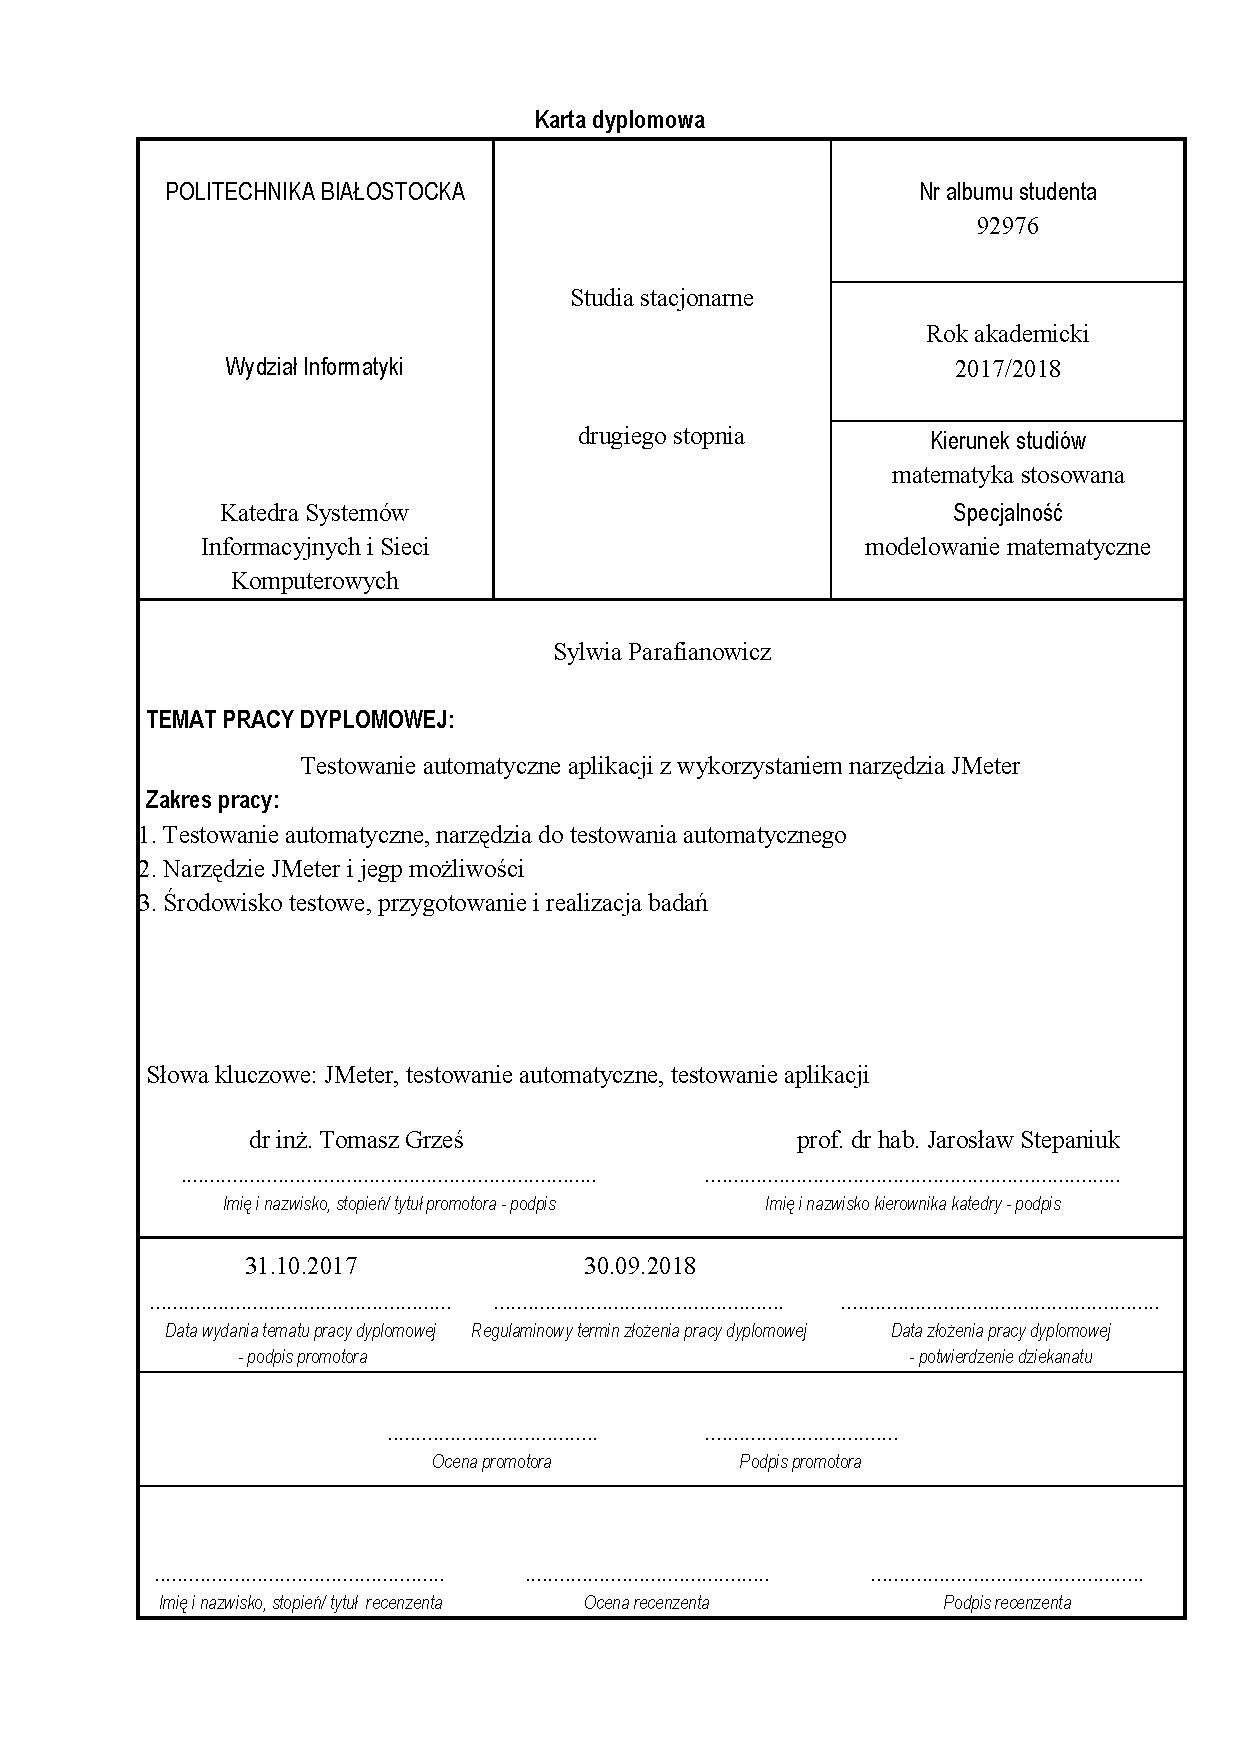
\includepdf[]{Karta.pdf}


\setcounter{page}{3}
\textbf{Thesis topic in English:} Automatic application testing using JMeter\\
\begin{center}
	\textbf{SUMMARY}
\end{center}

The purpose of this thesis is to show some interesting solution for a problem with choosing proper automation testing tools, especially for testing web applications. The idea is to use the most popular two: JMeter as a tool in which the test architecture is implemented and Selenium WebDriver for writing scripts in BeanShell Sampler (JMeter's component). The example of usage these tools is presented during testing a simple website on Wordpress.

\newpage

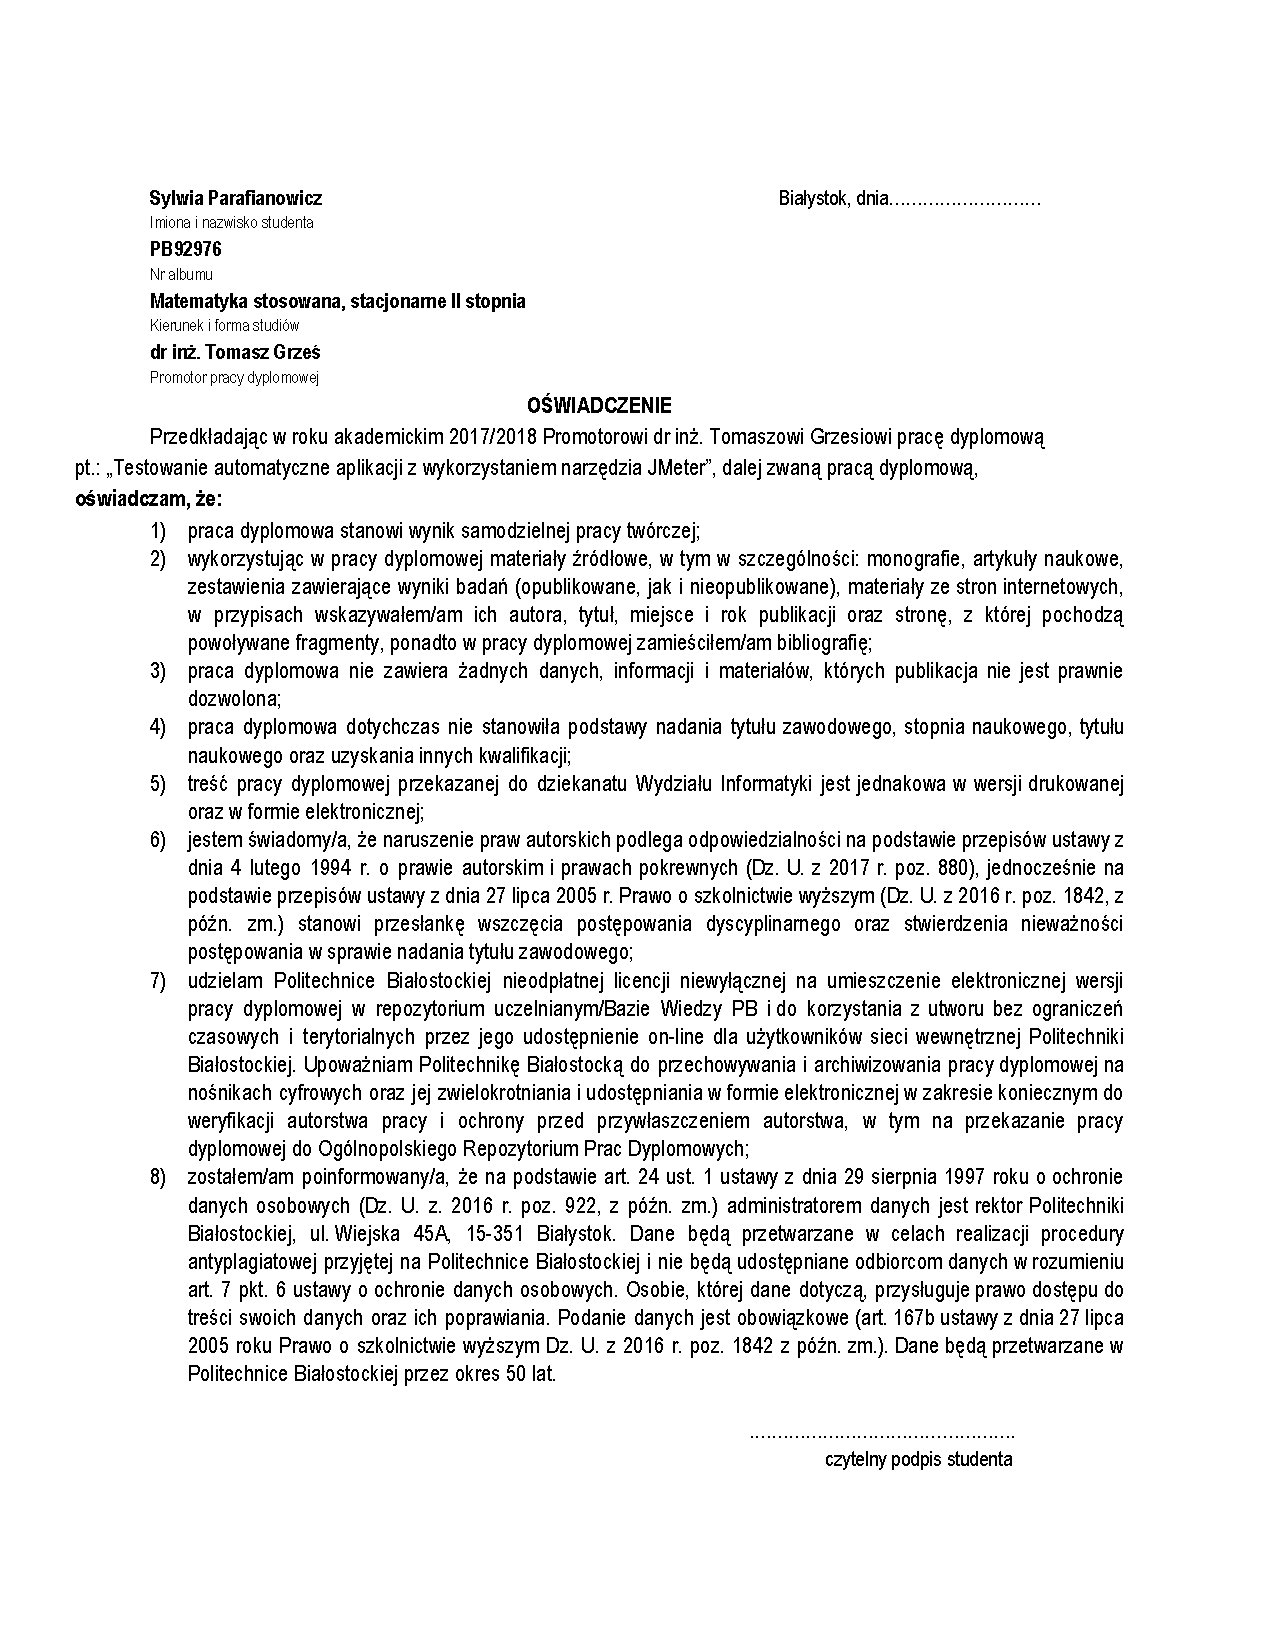
\includepdf[]{osw.pdf}

\setcounter{page}{5}
\tableofcontents

\newpage
\chapter{Wstęp} 


Automatyzacja testowania jest jednym ze sposobów testowania, który przy pomocy odpowiedniego oprogramowania wykonuje testy i porównuje aktualne rezultaty z oczekiwanymi. Ta technika testowania jest bardzo często wykorzystywana w projektach IT, ponieważ dzięki niej można znacznie dokładniej przetestować oprogramowanie niż gdyby to zrobić manualnie, a co za tym idzie zapewnia jego dostarczenie w znacznie krótszym czasie. Ponadto pozwala odciążyć testerów od wykonywania powtarzających się zadań. 


Jednym z kluczowych warunków do sukcesu przy wprowadzaniu automatyzacji procesu testowania jest dobór odpowiednich narzędzi. Celem niniejszej pracy jest wykorzystanie narzędzia JMeter w połączeniu z Selenium WebDriver do przetestowania aplikacji webowych, które wymagają bardzo wielu przypadków testowych i które są dobrymi kandydatami do automatyzacji. Ponadto, na podstawie przeprowadzonego eksperymentu, zostanie pokazane, że za pomocą tych dwóch narzędzi można w łatwy sposób stworzyć czytelne scenariusze testowe.  Rozwiązanie problemu zostanie zaprezentowane bazując na przykładowej stronie internetowej napisanej z użyciem platformy WordPress. 


Praca została podzielona na pięć rozdziałów. Pierwszy rozdział stanowi wstęp, w którym zaprezentowane zostają cele i motywacje stojące za niniejszą pracą. 


Drugi z nich zawiera definicje dotyczące testowania oprogramowania, w tym też testowania automatycznego, które wprowadzają w tematykę kolejnych rozdziałów. Zawiera też matematyczny aspekt w pracy - wspomniana definicja automatu skończonego.


Kolejny rozdział dotyczy opisu wszystkich programów, jakie będą wykorzystywane w pracy, wraz z krótkim uzasadnieniem ich wyboru w ostatnim podrozdziale. 


Czwarty rozdział stanowi część badawczą - przedstawia środowisko testowe, napisane dla niego przypadki testowe (z ang. \textit{test-cases}) oraz wyniki przeprowadzonych testów automatycznych. Podkreślony zostaje fakt, iż niniejszy eksperyment nie wyczerpuje tematyki pracy, a raczej przedstawia proponowane rozwiązanie na prostym przykładzie strony internetowej.

W ramach ostatniego rozdziału zawarto podsumowanie otrzymanych rezultatów z wyciągniętymi wnioskami i propozycjami rozwinięcia tematyki pracy w przyszłości.


\chapter{Wprowadzająca terminologia} \ \ \

\input r_11


\bigskip \bigskip

\input r_12



\chapter{Oprogramowania wykorzystywane w pracy} \ \ \

\input r_21

\bigskip \bigskip




\chapter{Środowisko testowe i przeprowadzone badania} \ \ \


\input r_31

\bigskip \bigskip

\input r_32



\newpage
\chapter{Podsumowanie} 

Postawioną tezą dla niniejszej pracy było pokazanie rozszerzonych możliwości JMetera jako narzędzia nie tylko do testów wydajnościowych, ale także do pisania automatycznych testów funkcjonalnych, wspomagając się skryptami pisanymi w Selenium WebDriver. Cel został osiągnięty - rezultat eksperymentu opisano dokładnie w poprzednim rozdziale.

Oczywiście, badania te nie wyczerpują tematu automatyzacji testowania za pomocą JMetera wraz z Selenium, lecz do realizacji wyznaczonych w pracy celów są wystarczające. Można rozszerzyć zastosowania tej koncepcji o następujące kwestie:
\begin{itemize}
\item dodanie kroków testowych związanych z zapytaniami bazodanowymi;
\item testowanie wydajności aplikacji webowych wspomagając się skryptami Selenium;
\item wykorzystanie niniejszego rozwiązania do testowania projektów, które wymaga interakcji z większą ilością interfejsów czy systemów, wykorzystując dodatkowe protokoły, takie jak JDBC, HTTP czy SOAP;
\item współdziałanie ze środowiskiem ciągłej integracji (ang. \textit{continuous integration}), takim jak Jenkins czy Travis CI;
\item współpraca z systemami kontroli wersji, takimi jak GIT czy SVN.
\end{itemize}





\newpage

\addcontentsline{toc}{chapter}{Bibliografia} 
\begin{thebibliography}{99}
\bibitem{aut}Anderson B., Witryna internetowa.  \emph{\url{https://medium.com/@briananderson2209/best-automation-testing-tools-for-2018-top-10-reviews}}, stan: 17.06.2018 r.
\bibitem{jmeter}Apache Software Foundation. Witryna internetowa. 
\emph{\url{http://jmeter.apache.org/usermanual/}}, stan: 28.05.2018 r.
\bibitem{comp}Apache Software Foundation. Witryna internetowa. \emph{\url{https://jmeter.apache.org/usermanual/component_reference.html}}, stan: 13.06.2018 r.

\bibitem{myers}Badgett T., Myers G. J., Sandler C., Thomas T. D., \emph{The art of software testing}, 1979
\bibitem{beanshell}BeanShell. Witryna internetowa. \emph{\url{http://www.beanshell.org/intro.html}}, stan: 12.09.2018 r.
\bibitem{webapp}Chaffee A., Witryna internetowa. \emph{\url{http://www.jguru.com/faq/view.jsp?EID=129328}}, stan: 12.09.2018 r.
\bibitem{ieee}\emph{IEEE 289 Standard for Software and System Test Documentation, IEEE Computer Society, 2008}
\bibitem{auto}\emph{IEEE 610.12:1990 Standard Glossary of Software Engineering Terminology, IEEE Computer Society}, 1990
\bibitem{succ} International Software Testing Qualifications Board, \emph{ISTQB - Certified Tester, Expert Level Syllabus - Test Automation - Engineering}, 2014
\bibitem{io} Mantyla M., Rafi D. M., Moses K. R. K., Peterson K., \emph{Benefits and Limitations of Automated Software Testing: Systematic Literature
Review and Practitioner Survey}, 2012.
\bibitem{bs} Niemeyer P., Witryna internetowa. \emph{\url{http://www.beanshell.org/intro.html}}, stan: 17.06.2018 r.
\bibitem{joomla} Oficjalna strona platformy Joomla!, Witryna internetowa, \emph{\url{https://www.joomla.org/about-joomla.html}}, stan: 28.09.2018 r.
\bibitem{lr} Oficjalna strona MicroFocus, \emph{\url{https://software.microfocus.com/en-us/products/loadrunner-load-testing/overview}}, stan: 29.09.2018 r.
\bibitem{stat}Oficjalna strona W3Techs, \emph{\url{https://w3techs.com/technologies/overview/content_management/all}}, stan: 29.09.2018 r.
\bibitem{wpa}Oficjalna strona platformy WordPress. Witryna internetowa. \emph{\url{https://wordpress.org/about/}}, stan: 20.09.2018 r.
\bibitem{roman}Roman A., \emph{Testowanie i jakość oprogramowania}, PWN, Warszawa, 2007
\bibitem{zmitr}Roman A., Zmitrowicz K., \emph{Testowanie oprogramowania w praktyce}, PWN, Warszawa 2017
\bibitem{selenium}SeleniumHQ. Witryna internetowa. \emph{\url{https://www.seleniumhq.org/}}, stan: 12.09.2018 r.
\bibitem{przypadek}SJSI. Witryna internetowa.\emph{\url{http://sjsi.org/slowo/przypadek-testowy/}}, stan: 16.09.2018 r.
\bibitem{smiglin}Smilgin R., \emph{Zawód tester}, PWN, Warszawa, 2016
\bibitem{istqb}SJSI, Witryna internetowa, \emph{\url{http://sjsi.org/slowo/testowanie-bialoskrzynkowe/}}, stan: 16.09.2018 r.



\end{thebibliography}


\addcontentsline{toc}{chapter}{Spis rysunków}
\begingroup
  \let\captionlinebreak\relax
  \listoffigures
\endgroup

\addcontentsline{toc}{chapter}{Spis tabel}
\listoftables

\end{document}